\documentclass{beamer}

\usetheme{metropolis}
\usepackage{natbib}
\usepackage{ulem}
\usepackage{amsmath}
\usepackage{amsthm}
\usepackage{amsfonts}
\usepackage{bm}
\usepackage{mathtools}
\usepackage{ifthen}

\newtheorem{proposition}{Proposition}
\newtheorem{assumption}{Assumption}

\theoremstyle{remark}
\newtheorem*{remark}{Remark}

\setbeamercolor{background canvas}{bg=white}

\setbeamercolor{normal text}{fg=black}
\setbeamercolor{frametitle}{bg=black, fg=white}

%%%%% macros -----------------------------------------------------------------------------

\renewcommand{\c}{\bm c}
\newcommand{\x}{\bm x}
\newcommand{\C}{\bm C}
\newcommand{\X}{\bm X}
\newcommand{\Z}{\bm Z}
\newcommand{\Xhat}{\widehat{\X}}
\newcommand \R {\mathbb{R}}

% RDPG stuff

\renewcommand{\S}{\widehat S}
\newcommand{\U}{\widehat{\bm U}}
\newcommand{\Spop}{S}
\newcommand{\Upop}{\bm U}

% mediator regression coefficients

\newcommand{\thetazero}{\bm \theta_0}
\newcommand{\thetat}{\bm \theta_\text{t}}
\newcommand{\Thetac}{\bm \Theta_\text{c}}
\newcommand{\Thetatc}{\bm \Theta_\text{tc}}

% mediator regression estimators

\newcommand \thetazerohat [1] {\widehat{\bm \theta}_0 \paren*{#1}}
\newcommand \thetathat [1] {\widehat{\bm \theta}_\text{t} \paren*{#1}}
\newcommand \Thetachat [1] {\widehat{\bm \Theta}_\text{c} \paren*{#1}}
\newcommand \Thetatchat [1] {\widehat{\bm \Theta}_\text{tc} \paren*{#1}}

% outcome regression coefficients

\newcommand{\betazero}{\beta_0}
\newcommand{\betat}{\beta_\text{t}}
\newcommand{\betac}{\beta_\text{c}}
\newcommand{\betax}{\beta_\text{x}}

% outcome regression estimators

\newcommand \betazerohat [1] {\widehat{\beta}_0 \paren*{#1}}
\newcommand \betathat [1] {\widehat{\beta}_\text{t} \paren*{#1}}
\newcommand \betachat [1] {\widehat{\beta}_\text{c} \paren*{#1}}
\newcommand \betaxhat [1] {\widehat{\beta}_\text{x} \paren*{#1}}

\newcommand \xihat [1] {\widehat{\xi} \paren*{#1}}

% causal estimands

\newcommand{\ate}{\Psi_\text{ate} \paren*{t, t^*}}
\newcommand{\cde}{\Psi_\text{cde} \paren*{t, t^*, \x}}
\newcommand{\nde}{\Psi_\text{nde} \paren*{t, t^*}}
\newcommand{\nie}{\Psi_\text{nie} \paren*{t, t^*}}

\newcommand \cdehat [1] {\widehat{\Psi}_\text{cde} \paren*{#1}}
\newcommand \ndehat [1] {\widehat{\Psi}_\text{nde} \paren*{#1}}
\newcommand \niehat [1] {\widehat{\Psi}_\text{nie} \paren*{#1}}

\newcommand{\RDPG}{\operatorname{RDPG}}
\newcommand \cond {\mid}
\newcommand \dist {\sim}

\DeclarePairedDelimiter{\paren}{(}{)}
\DeclarePairedDelimiter{\set}{\{}{\}}
\DeclarePairedDelimiter{\brac}{[}{]}
\DeclarePairedDelimiter{\norm}{\lVert}{\rVert}

\newcommand{\dx}[1][]{%
   \ifthenelse{ \equal{#1}{} }
      {\ensuremath{\;\mathrm{d}x}}
      {\ensuremath{\;\mathrm{d}#1}}
}


\renewcommand{\P}[2][]{%
   \ifthenelse{ \equal{#1}{} }
      {\ensuremath{\mathbb{P} \brac*{#2}}}
      {\ensuremath{\mathbb{P} \brac*{#2 \mid #1}}}
}

\newcommand{\E}[2][]{%
   \ifthenelse{ \equal{#1}{} }
      {\ensuremath{\mathbb{E} \brac*{#2}}}
      {\ensuremath{\mathbb{E} \brac*{#2 \mid #1}}}
}

%%%%% end macros ------------------------------------------------------------------
\hypersetup{colorlinks,citecolor=cyan, urlcolor=cyan, linkcolor=black}

\title{Estimating indirect effects induced by homophily via spectral network regression}
\date{2022-07-07}
\author{Alex Hayes and Keith Levin}
\institute{University of Wisconsin-Madison}


\begin{document}

\maketitle

\begin{frame}{Setting}
    \begin{columns}
        \column{0.5\textwidth}

        \begin{figure}
            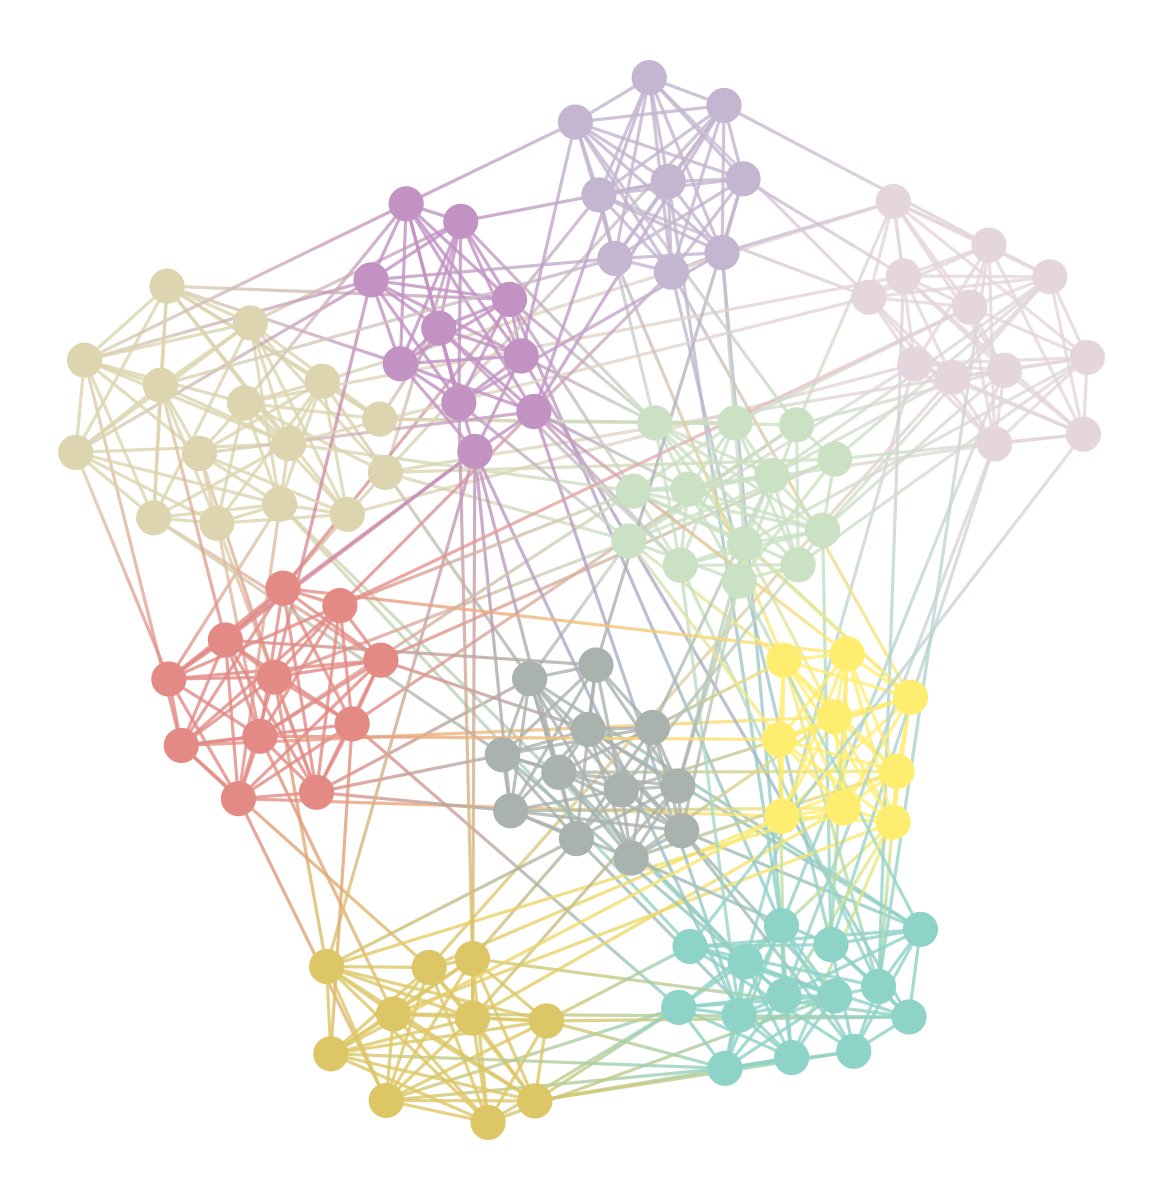
\includegraphics[width=\textwidth]{figures/assortative.png}
        \end{figure}

        \column{0.5\textwidth}

        Network $A \in \set{0, 1}^{n \times n}$

        Nodal covariates $\Z_1, ..., \Z_n \in \R^{p}$

        Nodal outcomes $Y_1, ..., Y_n \in \R$

    \end{columns}
\end{frame}

\begin{frame}{Regression incorporating network principle components}

    Regression with rank-$k$ truncated eigendecomposition of $A$

    \begin{align*}
        \E[U, S]{A}           & = \X \X^T                                               \\
        \E[\Z_i, U_i, S]{Y_i} & = \betazero + \Z_i \beta_\text{z} + \X_i \beta_\text{x}
    \end{align*}

    $\beta_\text{x}$ has a nice interpretation under stochastic blockmodels

\end{frame}


\begin{frame}{Network model: stochastic blockmodel (SBM)}
    \begin{columns}
        \column{0.5\textwidth}

        \begin{figure}
            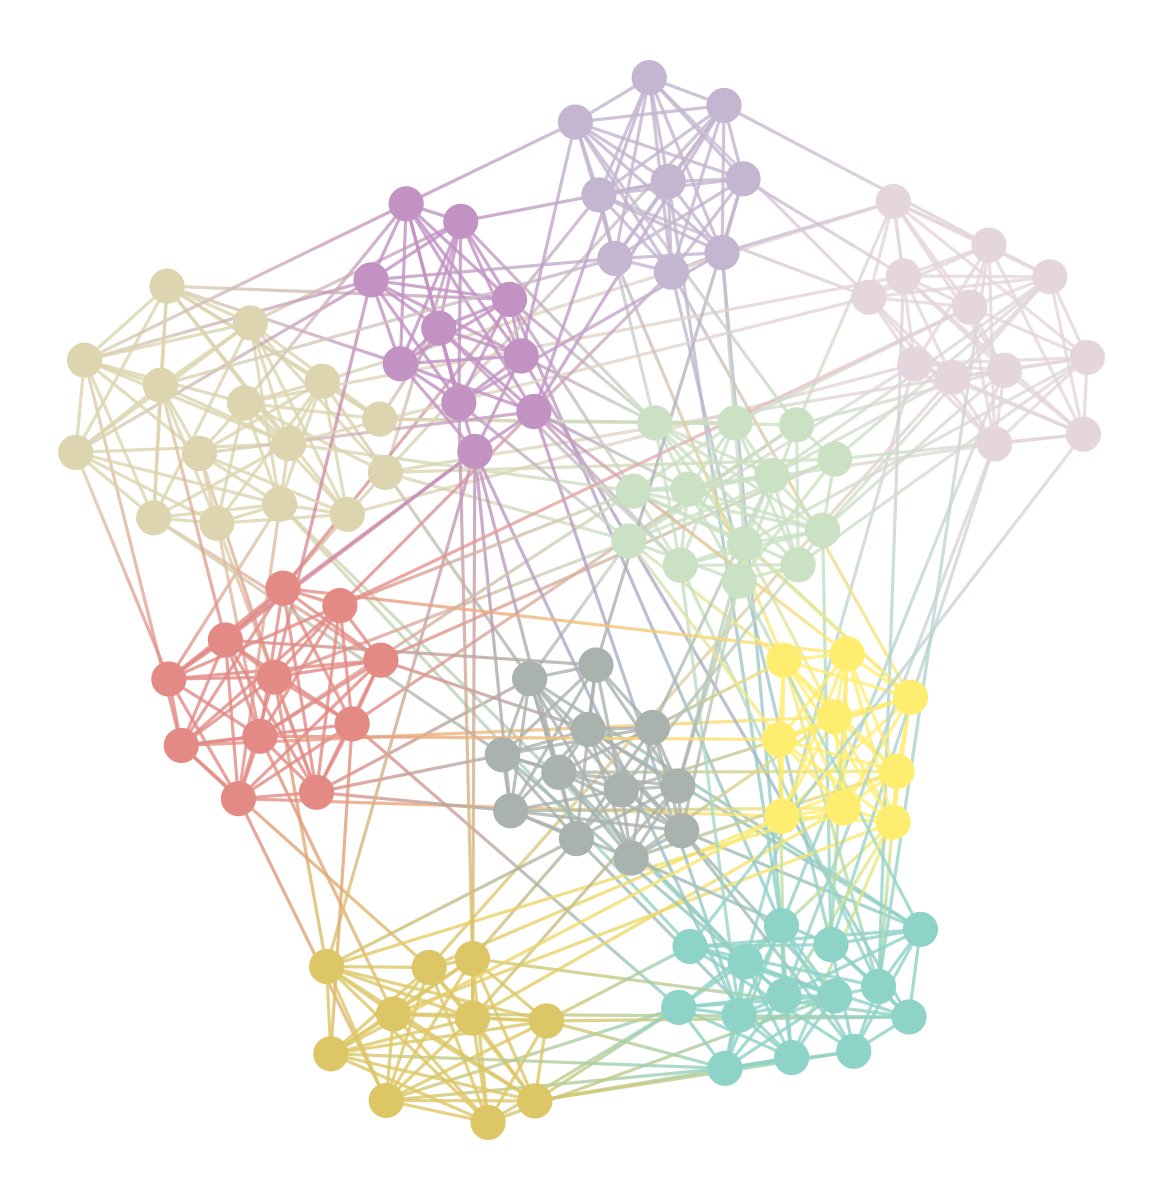
\includegraphics[width=\textwidth]{figures/assortative.png}
        \end{figure}

        \column{0.5\textwidth}

        \textbf{Degree-corrected SBM}

        \vspace{4mm}

        $k$ ``blocks'' or communities
        $B \in [0, 1]^{k \times k}$ inter-block edge probabilities

        \vspace{3mm}

        $w(i) \in \set{1, ...., k}$ node $i$'s block
        $\gamma_i \in [0, 1]$ node $i$'s popularity

        \begin{align*}
            \P[w, \gamma]{A_{ij} = 1} = \gamma_i \cdot B_{w(i), w(j)} \cdot \gamma_j
        \end{align*}

    \end{columns}
\end{frame}

\begin{frame}{Network model: broad generalization of the SBM}
    \begin{columns}
        \column{0.5\textwidth}

        \begin{figure}
            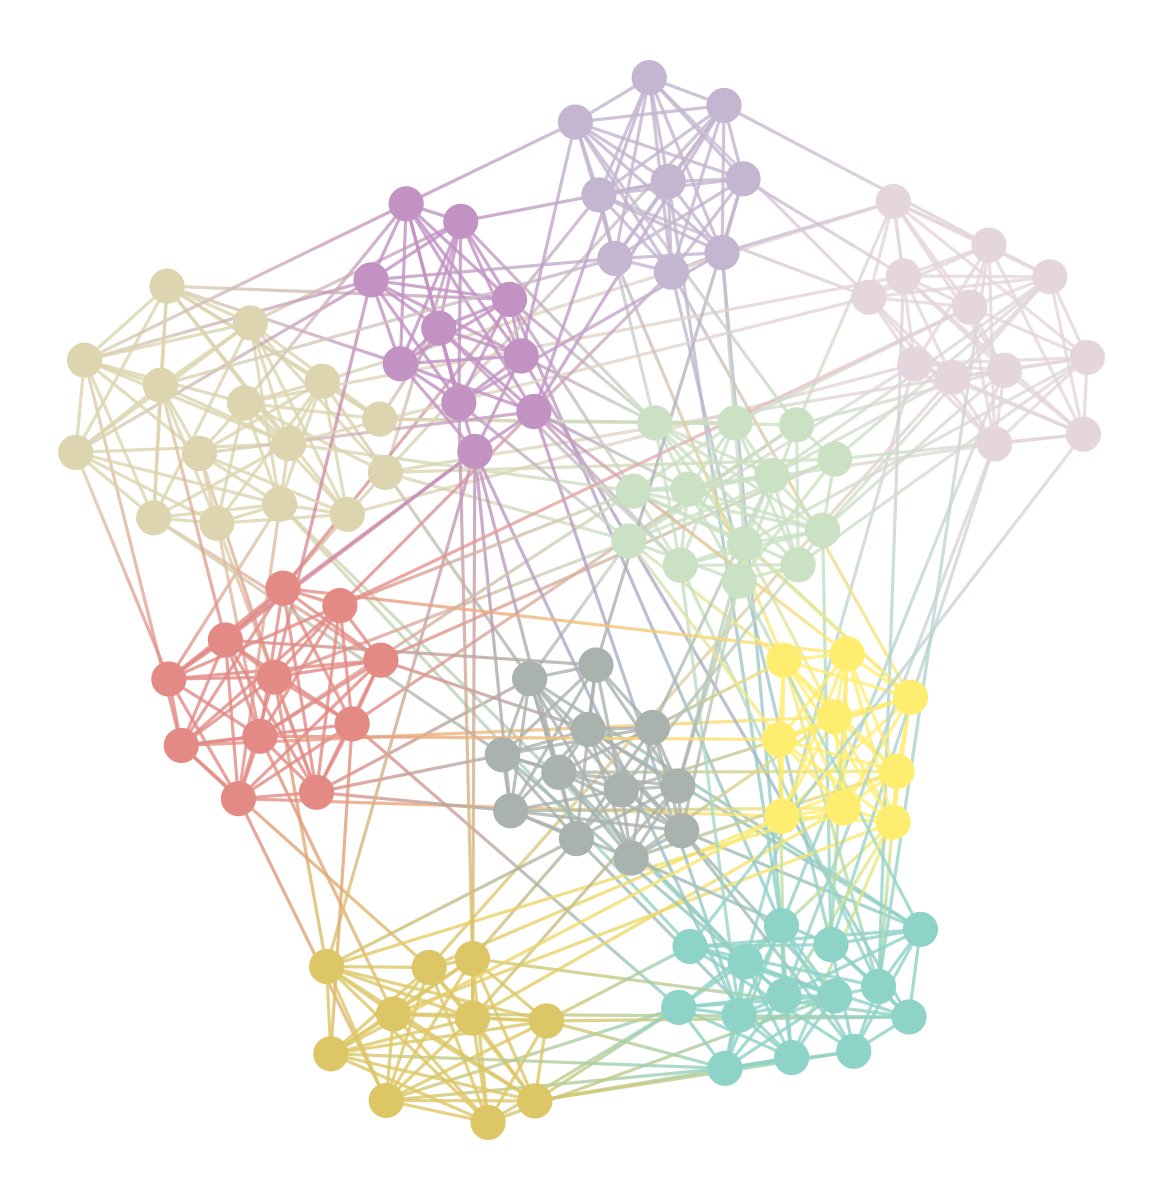
\includegraphics[width=\textwidth]{figures/assortative.png}
        \end{figure}

        \column{0.5\textwidth}

        Random dot product graphs

        \begin{align*}
            A_{ij} \cond \X & \dist \mathrm{Bernoulli} \paren*{\X_i^T \X_j} \\
            \X_i            & \dist F
        \end{align*}

        $F$ a $k$-dimensional inner-product distribution

        \begin{align*}
            (A, \X) \dist \RDPG(F,n)
        \end{align*}

    \end{columns}
\end{frame}

\begin{frame}{Random dot product graphs have low rank structure}
    \begin{columns}
        \column{0.5\textwidth}

        Population adjacency $\E[\X]{A}$

        \begin{figure}
            
\includegraphics[width=\textwidth]{figures/presentation/adjacency-population.png}
        \end{figure}

        \column{0.5\textwidth}

        Sample adjacency $A$

        \begin{figure}
            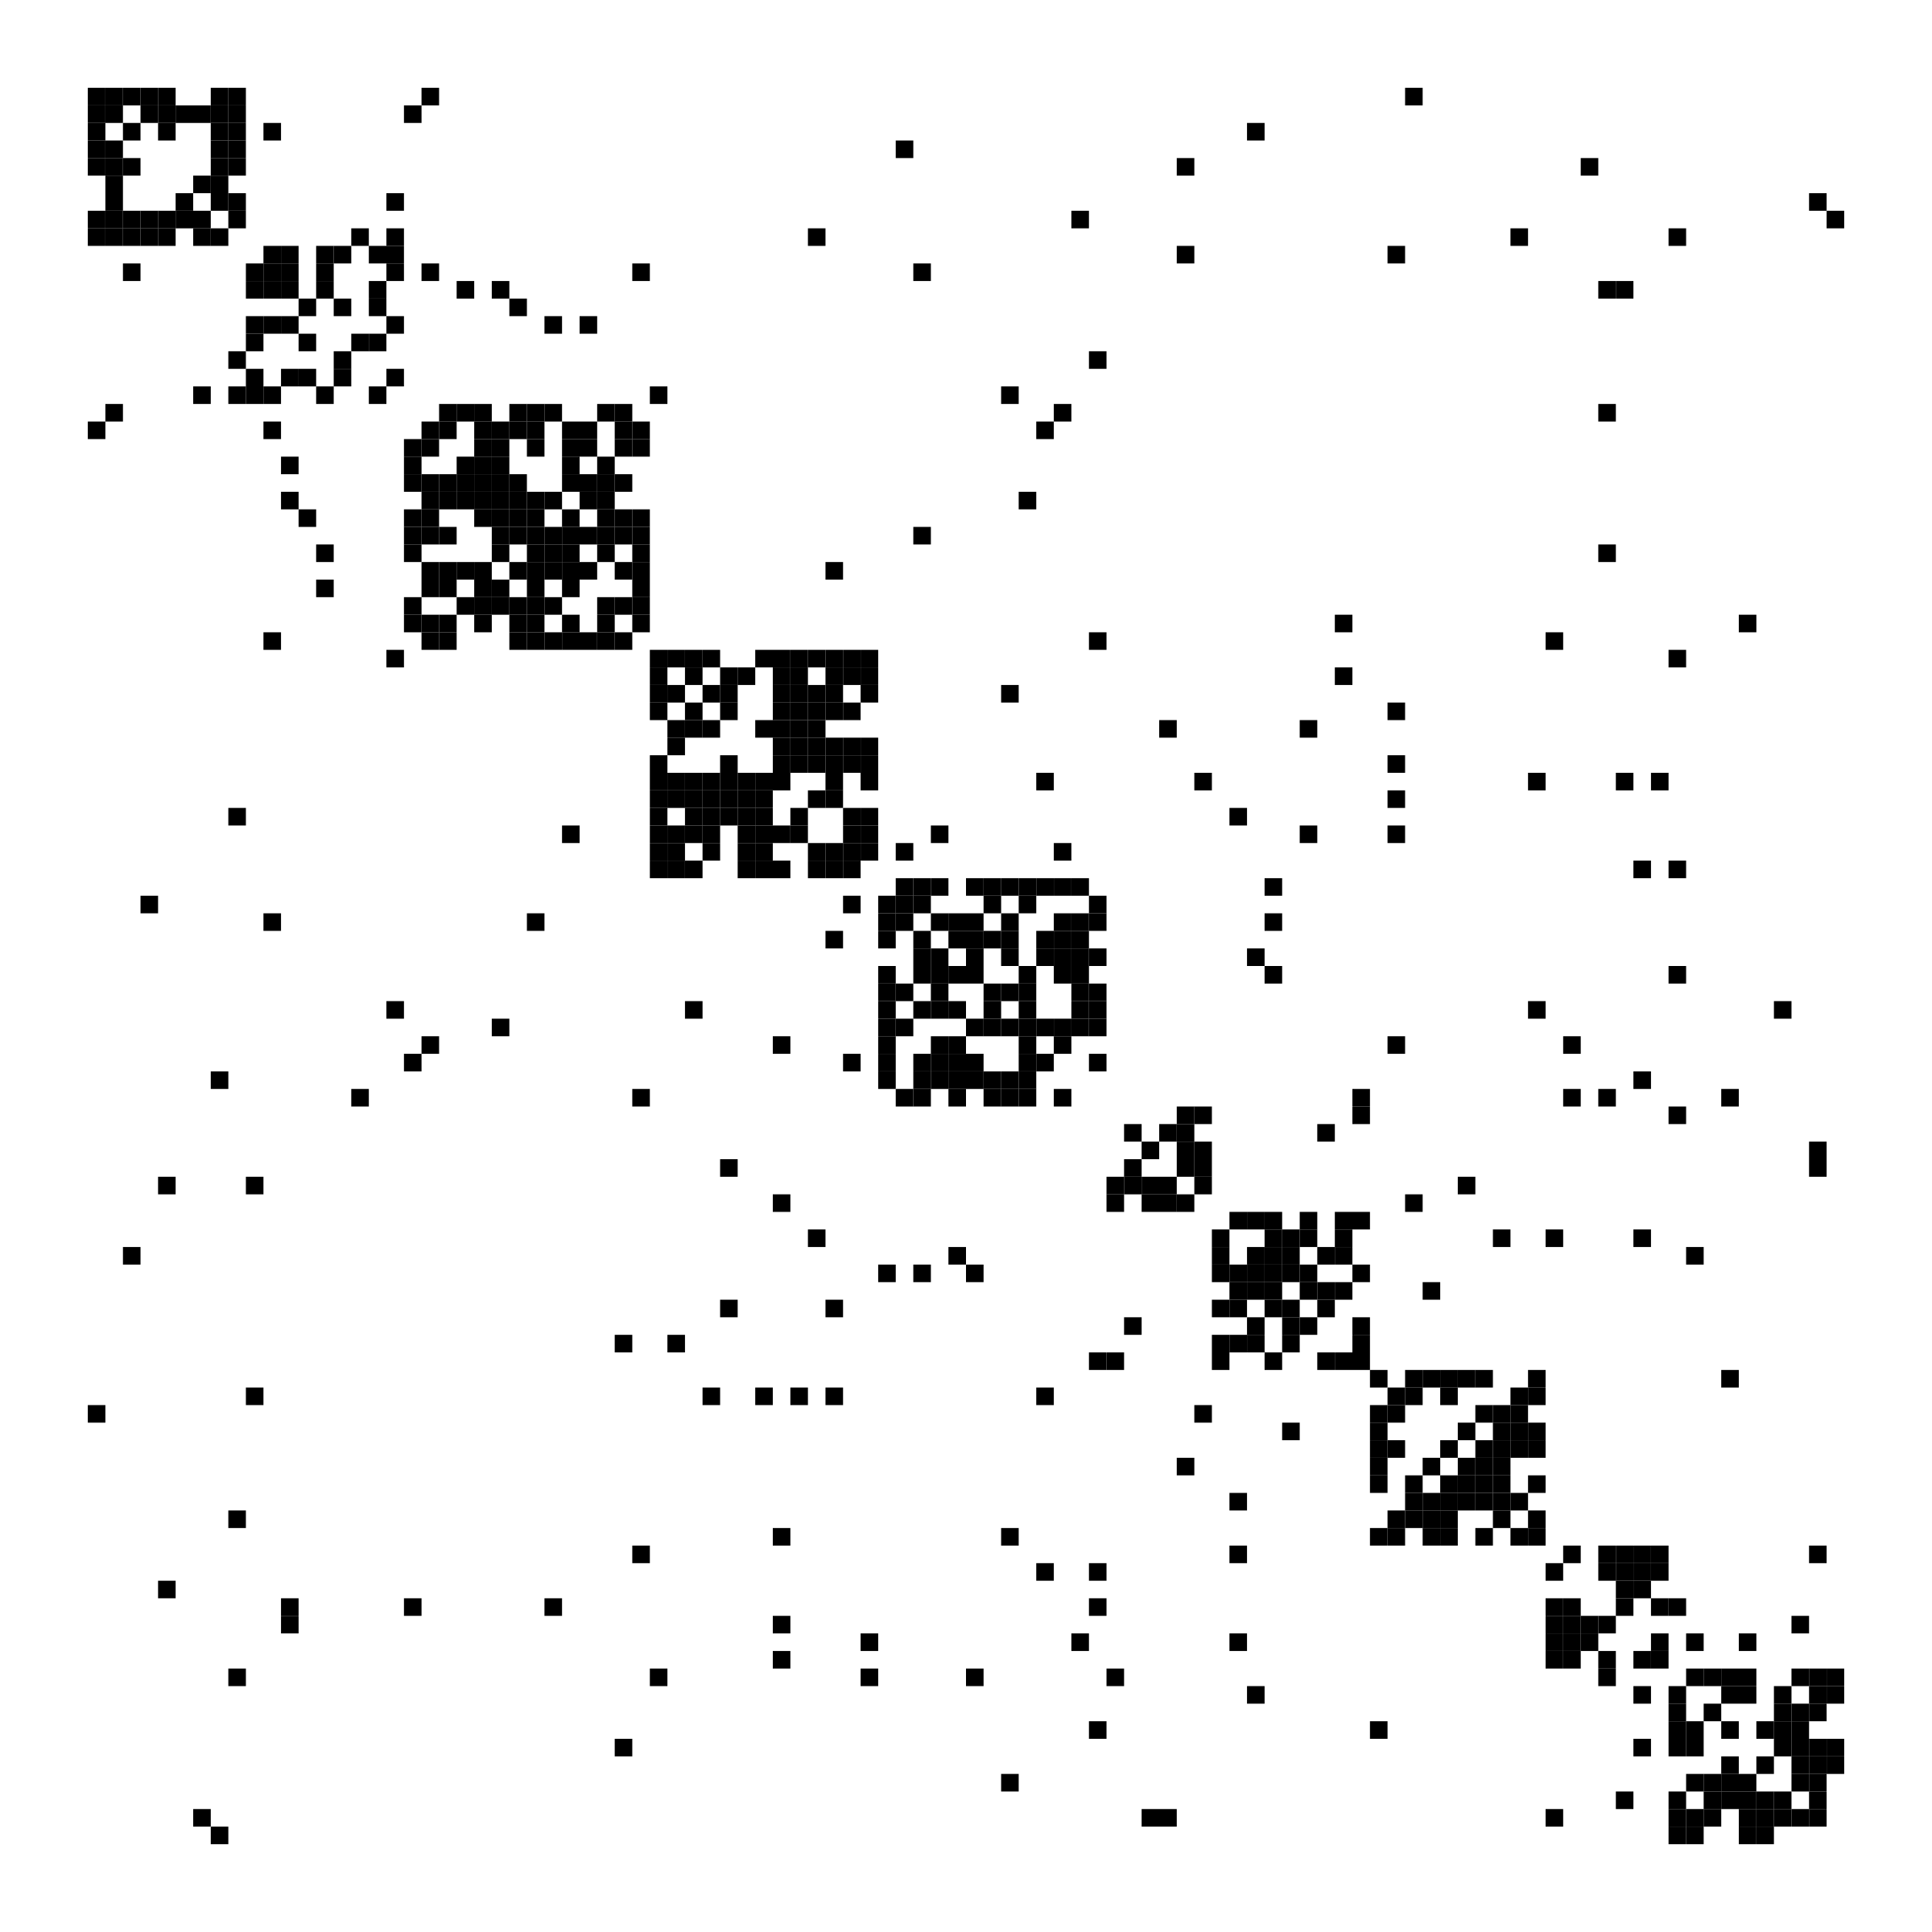
\includegraphics[width=\textwidth]{figures/presentation/adjacency-sample.png}
        \end{figure}

    \end{columns}

    \centering
    Stochastic block model with rank $k = 10$

\end{frame}

\begin{frame}{Adjacency spectral embedding}

    \begin{definition}[ASE]

        The \emph{adjacency spectral embedding} $\Xhat \in \R^{n \times k}$ of a network $A$ is defined as

        \begin{align*}
            \Xhat = \U \S^{1/2}
        \end{align*}

        \noindent where $A = \U \S \U^T$ is the rank $k$ truncated singular value decomposition of $A$.
    \end{definition}

    ``Principal components'' of a network

\end{frame}

\begin{frame}{Adjacency spectral embedding}

    \begin{lemma}[\cite{lyzinski_perfect_2015}, Lemma 5]
        \label{lem:2toinfty}

        Suppose that $(A, \X) \dist \RDPG(F,n)$. Then, letting $\Xhat_i \in \R^d$ denote the $i$-th row of $\Xhat$, there exists a universal constant $C$ and a sequence of orthogonal matrices $Q_n \in \R^{k \times k}$ such that eventually,

        \begin{equation*}
            \max_{i \in [n]} \, \norm*{Q_n \Xhat_i - \X_i} \le \frac{C \log n}{\sqrt n}.
        \end{equation*}

        This occurs even if $A$ is observed with sub-gamma noise \citep{levin_recovering_2022}.

    \end{lemma}
\end{frame}

\begin{frame}{Previous approaches to network regression}

    Regression with rank-$k$ truncated eigendecomposition of $A$

    \begin{align*}
        A                & = U S U^T                                               \\
        \E[\Z_i, A]{Y_i} & = \betazero + \Z_i \beta_\text{z} + \X_i \beta_\text{x}
    \end{align*}

    Why low rank network decompositions?

    $\beta_\text{x}$ roughly ``effect of being in block $w(i)$ with popularity $\gamma_i$''

    $\beta_\text{x}$ only identifiable up to rotation

\end{frame}

\begin{frame}{Regression incorporating network principle components}

    This has been done in \cite{le_linear_2021}!

    \begin{align*}
        \E[\Z_i, A]{Y_i} & = \Z_i \beta_\text{z} + \xi + \alpha
    \end{align*}

    Let $S_k$ be truncated eigenspace of $\E[\X]{A}$ and define $\mathcal R = \mathrm{col}(\Z) \cap S_k$. Require $\xi \in \mathcal R$, $\Z_i \beta_\text{z} \perp \mathcal R$ and $\alpha \perp \mathcal R$

    \begin{align*}
        \E[\Z_i, A]{Y_i} =
        \underbrace{\Z_i \beta_\text{z}}_\text{covariate effect} +
        \underbrace{\Z_i \theta}_\text{shared effect} +
        \underbrace{\alpha}_\text{network effect}
    \end{align*}
\end{frame}

\begin{frame}{AddHealth data from \cite{le_linear_2021}}

    \begin{itemize}
        \item Data on 2,152 high school students (nodes)
        \item 7,986 self-reported friendships (edges)
        \item Outcome: measure of mental health
        \item Covariates: race, sex, grade in school
    \end{itemize}

    \begin{columns}
        \column{0.5\textwidth}

        \begin{figure}
            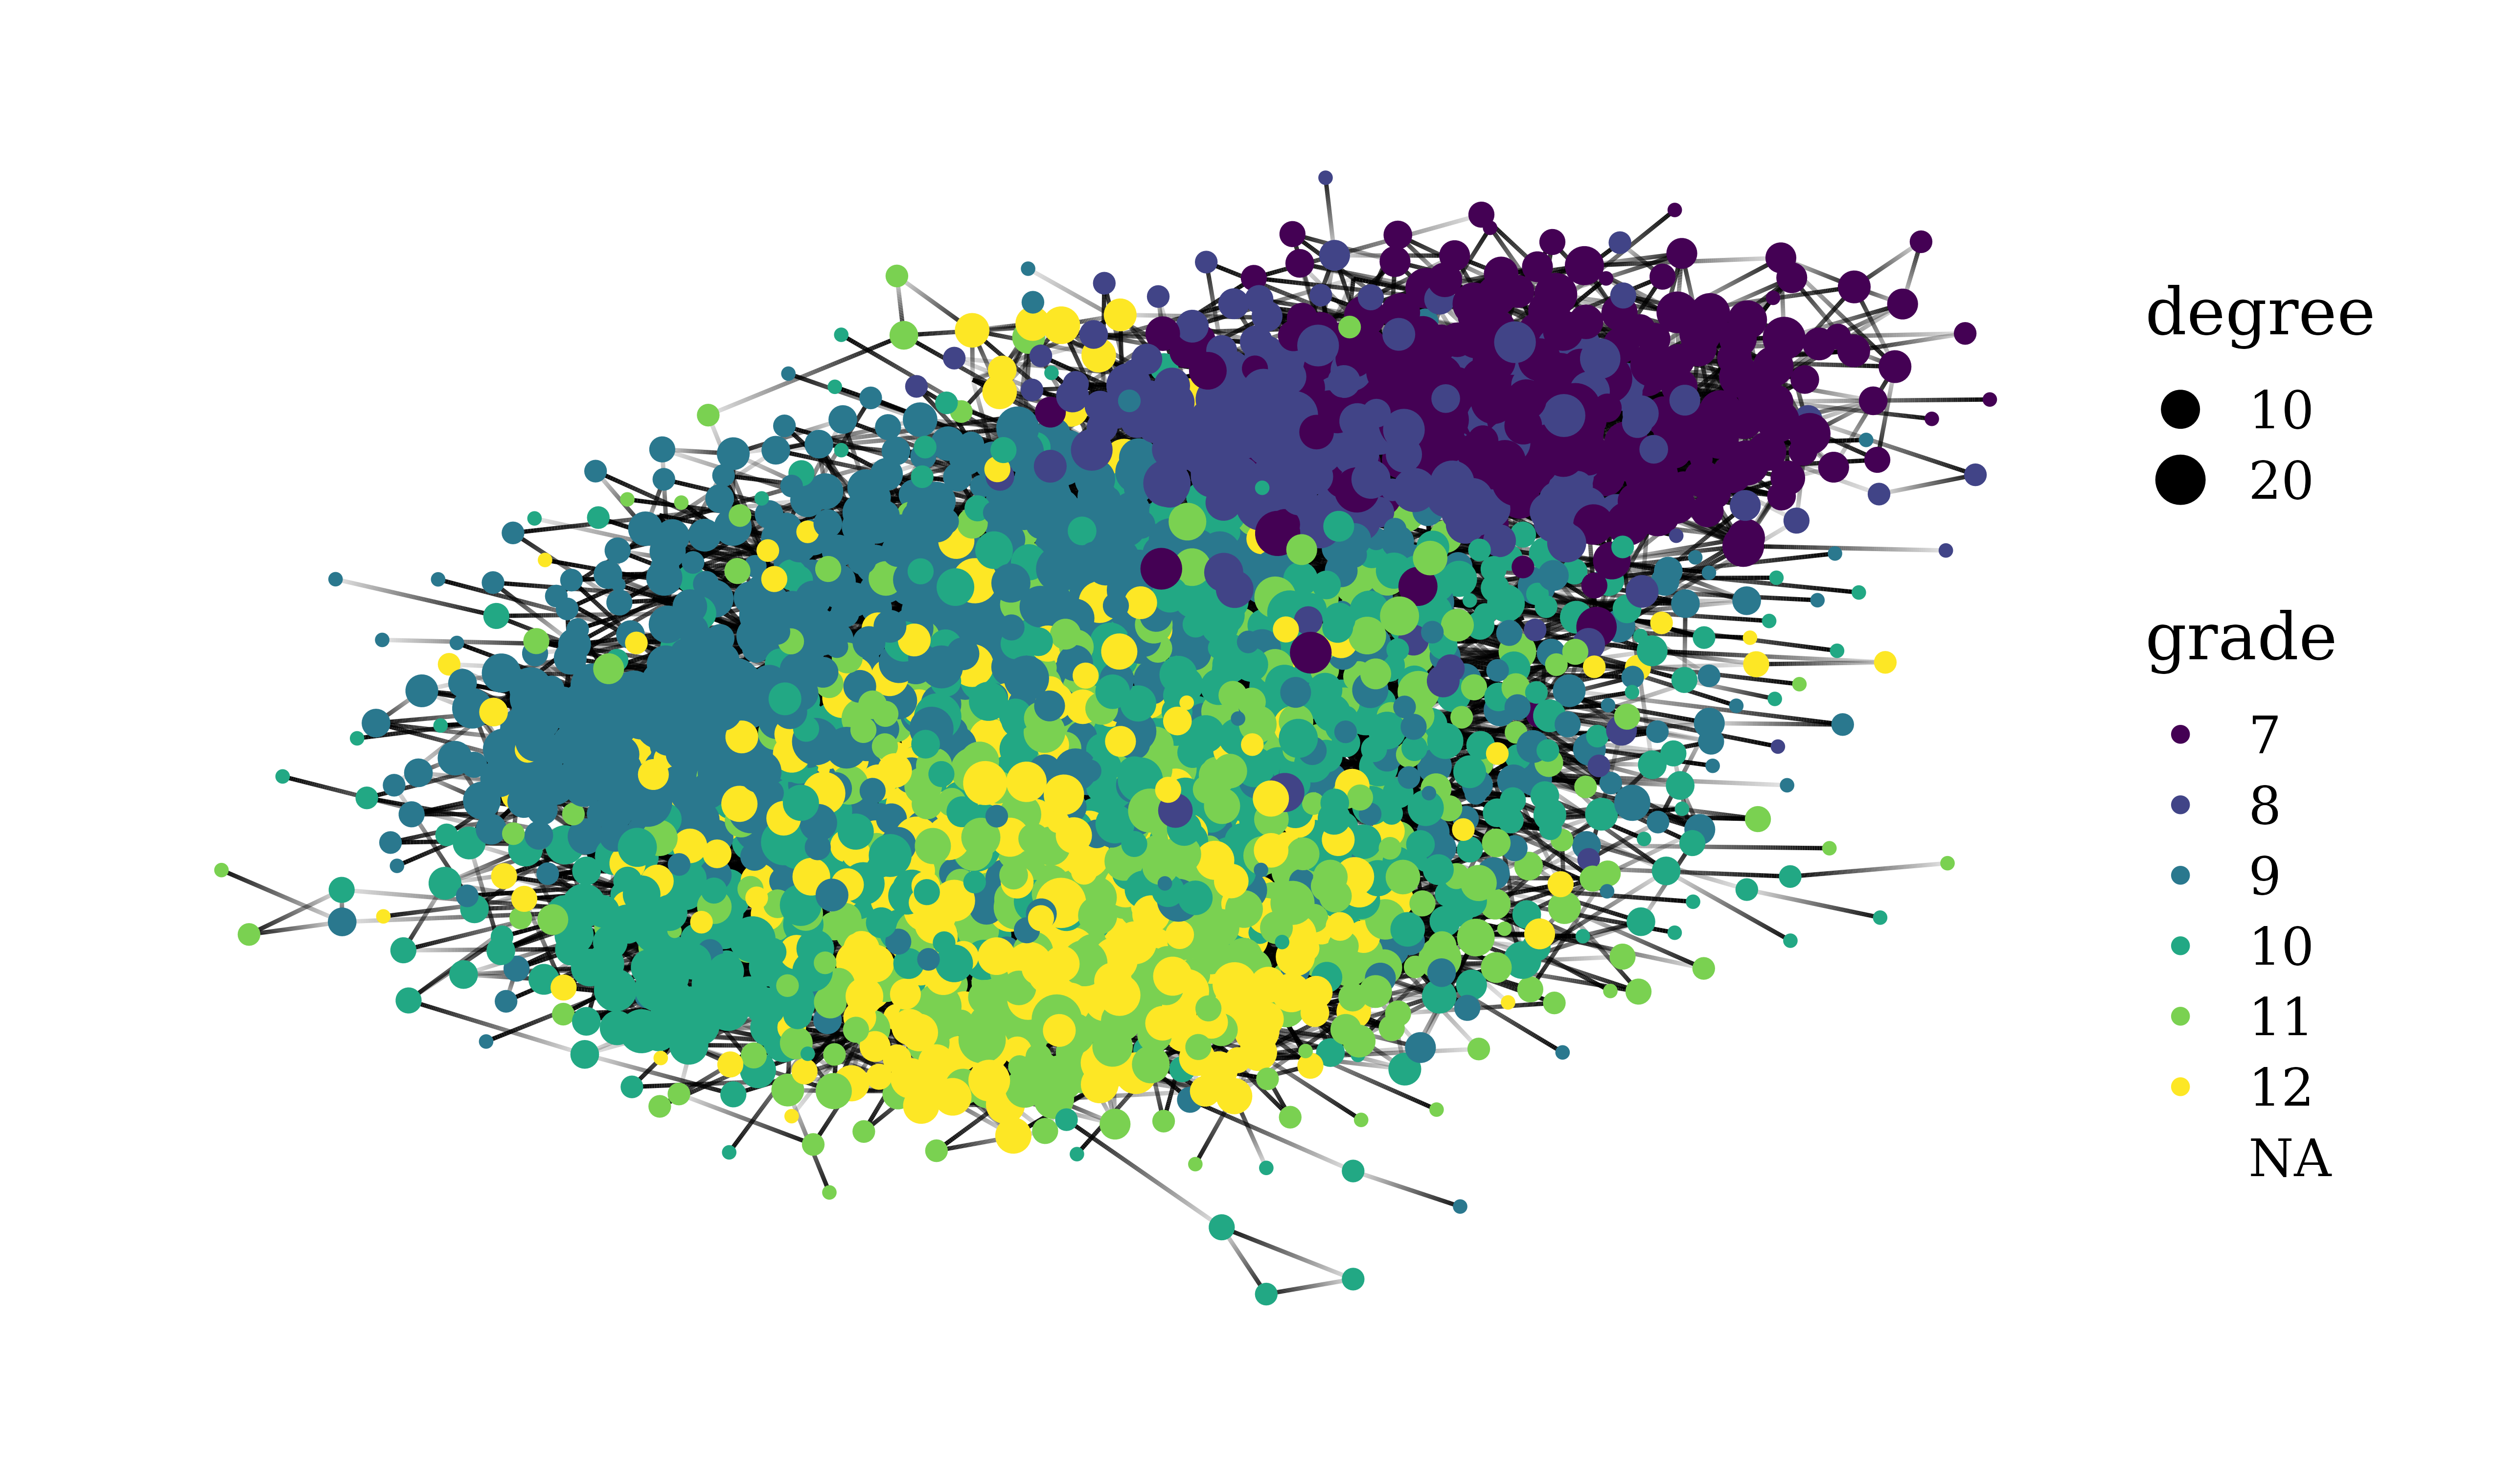
\includegraphics[width=\textwidth]{figures/presentation/homophily-grade.png}
            \caption{Grade based homophily in a high school social network.}
            \label{fig:homophily-grade}
        \end{figure}

        \column{0.5\textwidth}

        \begin{figure}
            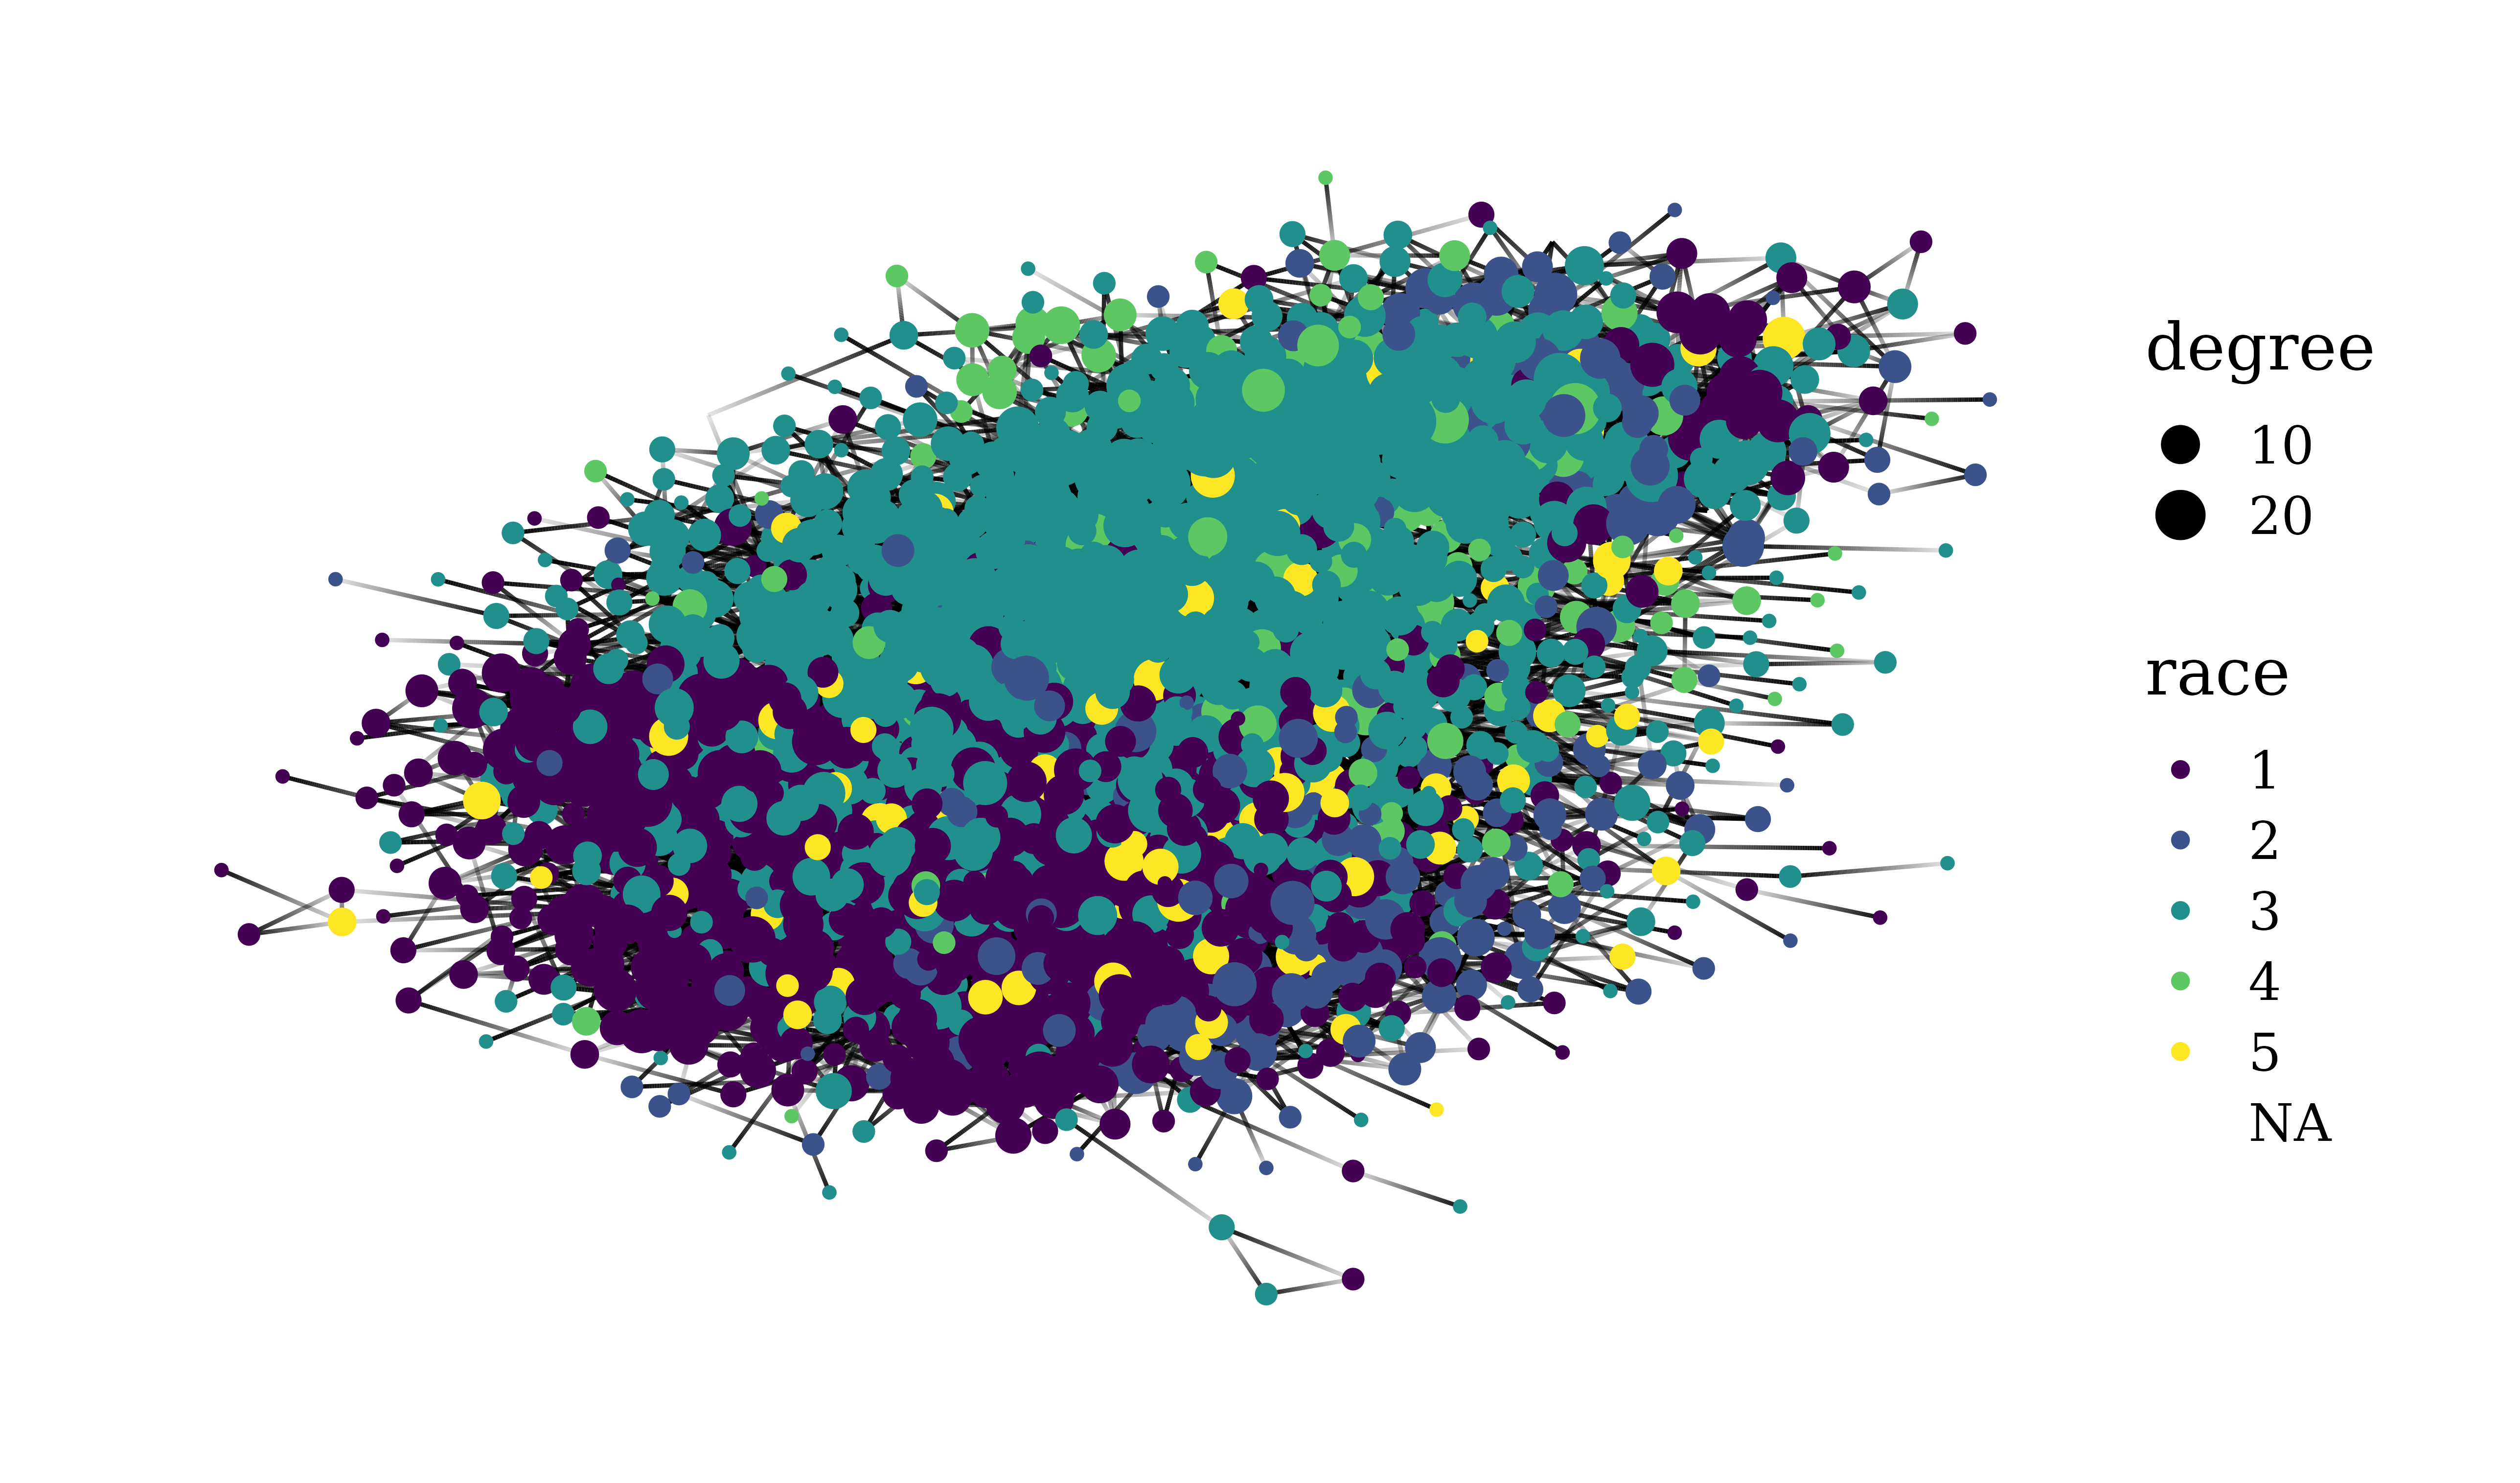
\includegraphics[width=\textwidth]{figures/presentation/homophily-race.png}
            \caption{Race based homophily in a high school social network.}
            \label{fig:homophily-race}
        \end{figure}

    \end{columns}
\end{frame}

\begin{frame}{Results when applied to AddHealth data}

    \begin{itemize}
        \item $k$ estimated to be 9
        \item $\mathrm{dim}(\mathcal R)$ estimated to be zero, no network-outcome confounding
        \item $\beta$: significant sex and grade effects
        \item $\beta$: weak effect of race, especially when compared to OLS estimates
    \end{itemize}

\end{frame}

\begin{frame}{Results when applied to AddHealth data: a mystery}

    \begin{itemize}
        \item $k$ estimated to be 9
        \item $\mathrm{dim}(\mathcal R)$ estimated to be zero, no network-outcome confounding
        \item $\beta$: significant sex and grade effects
        \item $\beta$: weak effect of race, especially when compared to OLS estimates
    \end{itemize}

    Why does controlling for latent position in network make the race effect go away?

    My hypothesis: race causes group membership, which in turn causes mental health outcomes, i.e. network position mediates rather than confounds race $\leftrightarrow$ mental health relationship

\end{frame}

\begin{frame}{Causal network regression}
    \begin{columns}
        \column{0.5\textwidth}

        \begin{figure}
            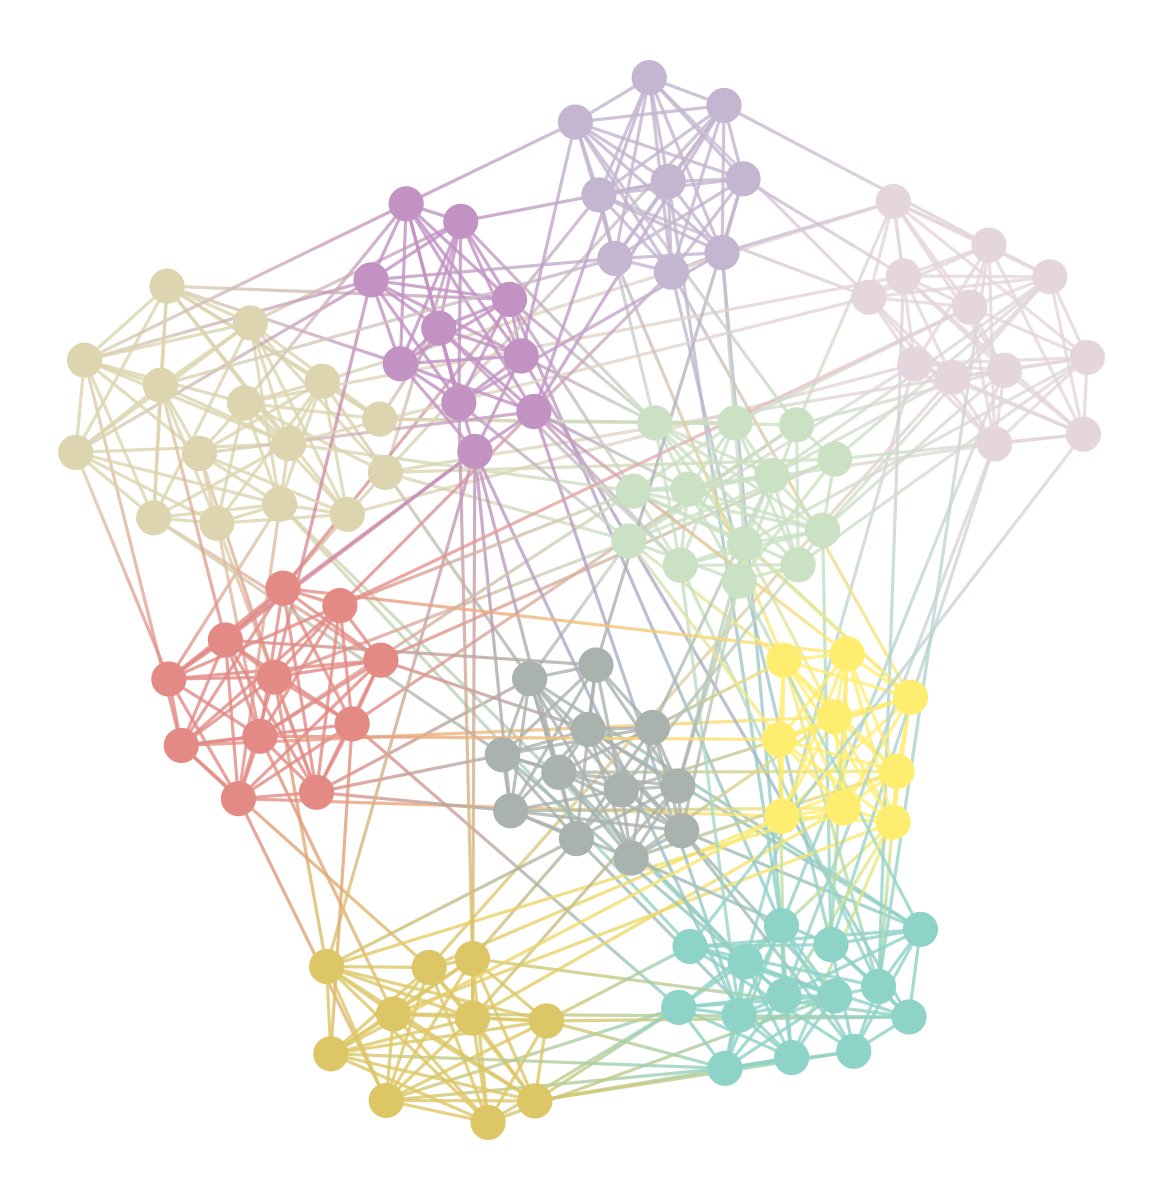
\includegraphics[width=\textwidth]{figures/assortative.png}
        \end{figure}

        \column{0.5\textwidth}

        Network $A \in \set{0, 1}^{n \times n}$

        Nodal covariates $\Z_1, ..., \Z_n \in \R^{p}$

        Nodal outcomes $Y_1, ..., Y_n \in \R$

        \vspace{6mm}

        Partition $\Z_i = (T_i, \C_i)$

        Treatment $T_i \in \set{0, 1}$

        Controls $\C_i \in \R^p$

        \vspace{6mm}

        No interference or contagion!
    \end{columns}
\end{frame}


\begin{frame}{Mediation in network-linked data for low-rank network models}

    \centering

    \begin{figure}
        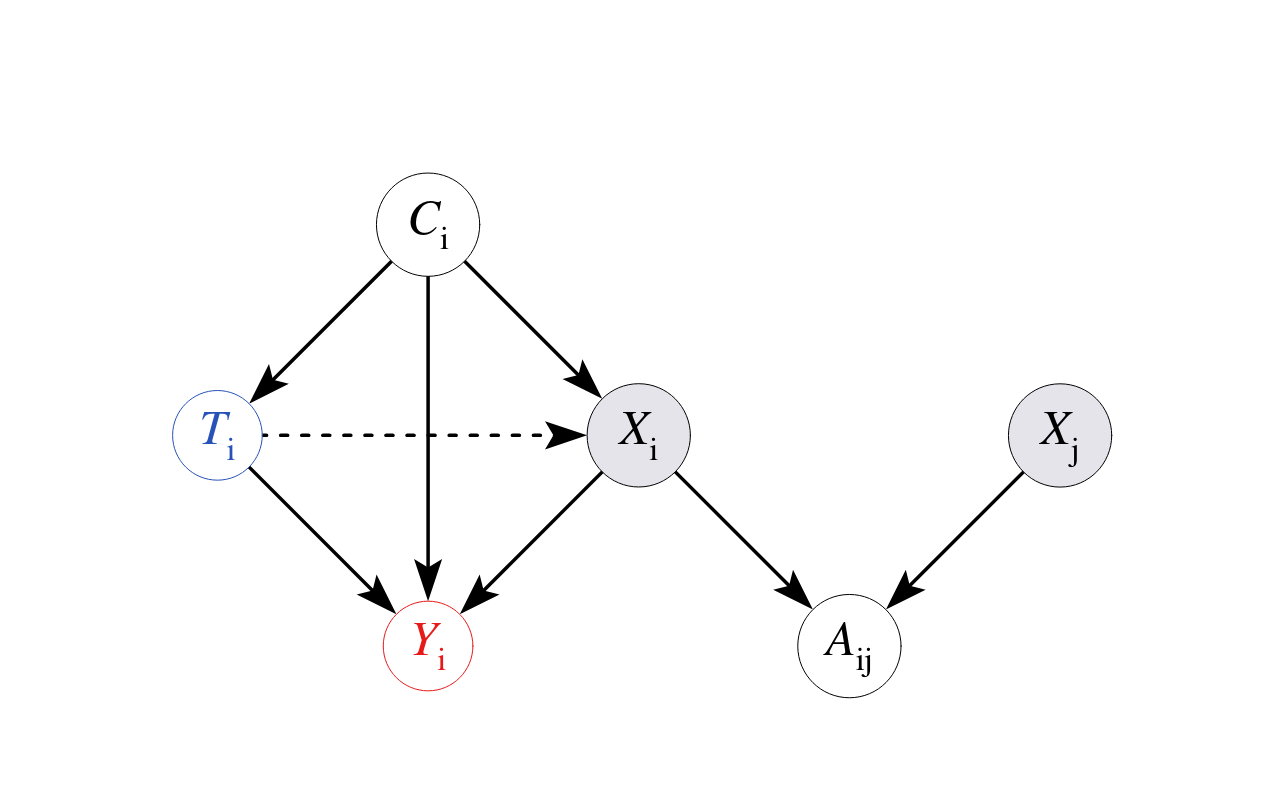
\includegraphics[width=0.9\textwidth]{figures/mediating.png}
        \caption{Directed acyclic graph (DAG) relating for node $i$ in a reduced rank network regression model. Portions of the DAG corresponding to nodes $j \neq i$ are omitted. $\X_i$ and $\X_j$ are not observed.}
        \label{fig:mediating}
    \end{figure}

\end{frame}

\begin{frame}{Causal estimands for mediated effects}

    There are a couple causal effects of interest
    \begin{align*}
         & \ate = \E{Y_t - Y_{t^*}} = \nde + \nie,                          \\
         & \cde = \E{Y_{t \, \x} - Y_{t^* \, \x}},                          \\
         & \nde = \E{Y_{t \, \X_{t^*}} - Y_{t^* \, \X_{t^*}}}, \text{ and } \\
         & \nie = \E{Y_{t \, \X_{t}} - Y_{t \, \X_{t^*}}}.
    \end{align*}

    Primarily interested in $\nde$ and $\nie$, natural direct and natural indirect effects.

\end{frame}

\begin{frame}{Non-parametric causal identification}

    \begin{proposition}[non-parametric identification, \cite{imai_identification_2010}]
        \label{prop:non-parametric-identification}

        Under our DAG (repeated below), $\nde$ and $\nie$ are identified, as

        \begin{align*}
            \label{eq:non-param-nested}
            \E{Y_{t \, \X_{t^*}}}
            = \iint \E[T = t, \c, \x]{y} \, p(\x \cond \c, T = t^*) \, p(\c) \dx[\x] \dx[\c].
        \end{align*}

    \end{proposition}

    i.e. under assumptions in DAG our \emph{counterfactual estimand} is strictly a function of \emph{observable functionals}

\end{frame}

\begin{frame}{Semi-parametric regression assumptions}

    Further, if

    \begin{align*}
        \underbrace{\E[T, \C, \X]{Y}}_{\mathbb R}
         & = \underbrace{\betazero}_{\mathbb R}
        + \underbrace{t}_{\{0, 1\}} \underbrace{\betat}_{\mathbb R}
        + \underbrace{\c}_{\mathbb R^{1 \times p}} \underbrace{\betac}_{\mathbb R^p}
        + \underbrace{\x}_{\mathbb R^{1 \times k}} \underbrace{\betax}_{\mathbb R^k} \\
        \underbrace{\E[T, \C]{\X}}_{\mathbb R^{1 \times k}}
         & = \underbrace{\thetazero}_{\mathbb R^{1 \times k}}
        + \underbrace{t}_{\{0, 1\}} \underbrace{\thetat}_{\mathbb R^{1 \times k}}
        + \underbrace{\c}_{\mathbb R^{1 \times p}} \underbrace{\Thetac}_{\mathbb R^{p \times k}}
    \end{align*}

    Then:

    \begin{align*}
        \cde & = \nde = \paren*{t - t^*} \, \betat      \\
        \nie & = \paren*{t - t^*} \, \thetat \, \betax.
    \end{align*}

\end{frame}

\begin{frame}{What this means for network regressions}

    Suppose the latent positions $\X$ are mediators. Then:

    \begin{itemize}
        \item $\betat$ is the \emph{natural direct effect} of $T$ on $Y$, not the average treatment effect
        \item If we compute a separate regression, we can compute the \emph{natural indirect effect} of $T$ on $Y$ (i.e. race causes group memberships causes mental health outcomes)
        \item These two effects add up to the average treatment effect
        \item Ordinary least squares \emph{ignoring the network structure} can be used to estimate the average treatment effect
    \end{itemize}

\end{frame}

\begin{frame}{A causal re-interpretation of \cite{le_linear_2021}'s results}

    Recall results (new causal interpretations in \textcolor{cyan}{cyan})

    \begin{itemize}
        \item $k$ estimated to be 9
        \item $\mathrm{dim}(\mathcal R)$ estimated to be zero, \sout{no network-outcome confounding} \textcolor{cyan}{race, grade and sex do not perfectly cause membership in any friend group}
        \item $\beta$: significant sex and grade \textcolor{cyan}{direct} effects
        \item $\beta$: weak \textcolor{cyan}{direct} effect of race estimated by network regression, strong \textcolor{cyan}{total} effect of race estimated by ordinary least squares $\implies$ large \textcolor{cyan}{indirect} effect of race
    \end{itemize}

\end{frame}

\begin{frame}{Constructing purpose-built causal estimators}

    Recall that we assume

    \begin{align*}
        \E[T, \C, \X]{Y}
         & = \betazero
        + t \, \betat
        + \c \, \betac
        + \x \, \betax  \\
        \E[T, \C]{\X}
         & = \thetazero
        + t \, \thetat
        + \c \, \Thetac
    \end{align*}

    and we want to estimate

    \begin{align*}
        \cde & = \nde = \paren*{t - t^*} \, \betat      \\
        \nie & = \paren*{t - t^*} \, \thetat \, \betax.
    \end{align*}

    Standard to fit two regressions and multiply coefficients to estimate indirect effect \citep{vanderweele_mediation_2014}


\end{frame}

\begin{frame}{Our estimator: plug ASE into ordinary least squares}

    Use least squares (with robust standard errors) to estimate the regression coefficients, then plug into causal estimators

    \begin{align*}
        \Z = \begin{bmatrix}
            1 & T & \C \\
        \end{bmatrix} \in \R^{n \times (1 + 1 + p)}.
    \end{align*}

    For estimates $\Xhat$ of $\X$, possibly equal to $\X$ itself, we estimate $\thetazero$, $\thetat$, and $\Thetac$
    \begin{align*}
        \begin{bmatrix}
            \thetazerohat{\Xhat} \\
            \thetathat{\Xhat}    \\
            \Thetachat{\Xhat}
        \end{bmatrix}
        = \paren*{\Z^T \Z}^{-1} \Z^T \Xhat.
    \end{align*}
\end{frame}


\begin{frame}{Our idea: plug ASE into ordinary least squares}

    \begin{align*}
        \Z \paren*{\Xhat} = \begin{bmatrix}
            1 & T & \C & \Xhat \\
        \end{bmatrix} \in \R^{n \times (1 + 1 + p + k)}
    \end{align*}

    Then

    \begin{align*}
        \begin{bmatrix}
            \betazerohat{\Xhat} \\
            \betathat{\Xhat}    \\
            \betachat{\Xhat}    \\
            \betaxhat{\Xhat}
        \end{bmatrix}
        = \left[ \Z \paren*{\Xhat}^T  \Z \paren*{\Xhat} \right]^{-1} \Z \paren*{\Xhat}^T Y.
    \end{align*}
\end{frame}

\begin{frame}{Our idea: plug ASE into ordinary least squares}

    Plug estimates into standard product-of-coefficients estimator

    \begin{align*}
        \cdehat{\Xhat} & = \ndehat{\Xhat} = \paren*{t - t^*} \, \betathat{\Xhat}     \\
        \niehat{\Xhat} & = \paren*{t - t^*} \, \thetathat{\Xhat} \, \betaxhat{\Xhat}
    \end{align*}

\end{frame}

\begin{frame}{Theoretical results}
    \begin{theorem}[informal]
        Asymptotically, regression coefficients using $\Xhat$ and $\X$ converge to the same distribution under generic low-rank models for $A$ with i.i.d. sub-gamma noise
    \end{theorem}

    \begin{corollary}[informal]
        Regression coefficients based on $\Xhat$ are asymptotically normal and converge at $\sqrt n$-rates.
    \end{corollary}

    \begin{corollary}[informal]
        $\cdehat{\Xhat}$ and $\niehat{\Xhat}$ are asymptotically normal and converge at $\sqrt n$-rates.
    \end{corollary}
\end{frame}

\begin{frame}{Rotational unidentifiability of mediator coefficients}

    There exists some unknown orthogonal rotation $Q$ such that

    \begin{align*}
        \sqrt n
        \begin{pmatrix}
            \thetazerohat{\Xhat} Q^T - \thetazero \\
            \thetathat{\Xhat} Q^T - \thetat       \\
            \Thetachat{\Xhat} Q^T - \Thetac
        \end{pmatrix}
        \to
        \mathrm{Normal} \paren*{0, \Sigma_\theta}
    \end{align*}
\end{frame}

\begin{frame}{Rotational unidentifiability of outcome coefficients}

    There exists some unknown orthogonal rotation $Q$ (same as in last slide) such that

    \begin{align*}
        \sqrt n
        \begin{pmatrix}
            \betazerohat{\Xhat} - \betazero \\
            \betathat{\Xhat} - \betat       \\
            \betachat{\Xhat} - \betac       \\
            Q \, \betaxhat{\Xhat} - \betax
        \end{pmatrix}
        \to
        \mathrm{Normal} \paren*{0, \Sigma_\beta}
    \end{align*}

    Rotational unidentifiability of $\betax$ and $\thetat$ cancel each other out in causal estimator for $\nie$!
\end{frame}

\begin{frame}{Re-analyzing the AddHealth data with our estimators}

    \centering

    \begin{figure}
        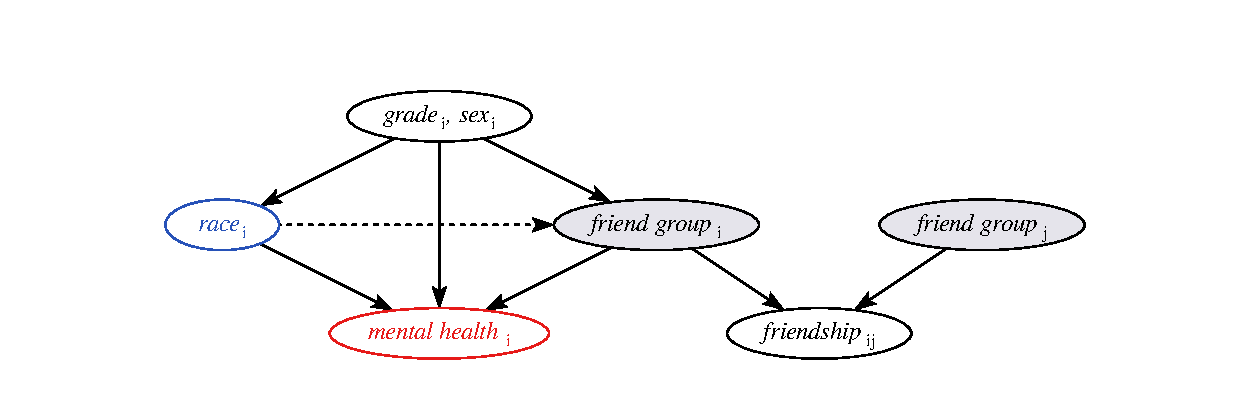
\includegraphics[width=\textwidth]{figures/addhealth-dag.pdf}
        \caption{Assumptions about the causal structure of the AddHealth data}
        \label{fig:addhealth-dag}
    \end{figure}

    Estimation: need to choose dimension $k$ of spectral embedding

\end{frame}

\begin{frame}{Choosing the rank of the network}

    \begin{itemize}
        \item Use cross-validated eigenvalues by \cite{chen_estimating_2021}
        \item Check sensitivity of results to choice of $k$
    \end{itemize}

    \begin{figure}
        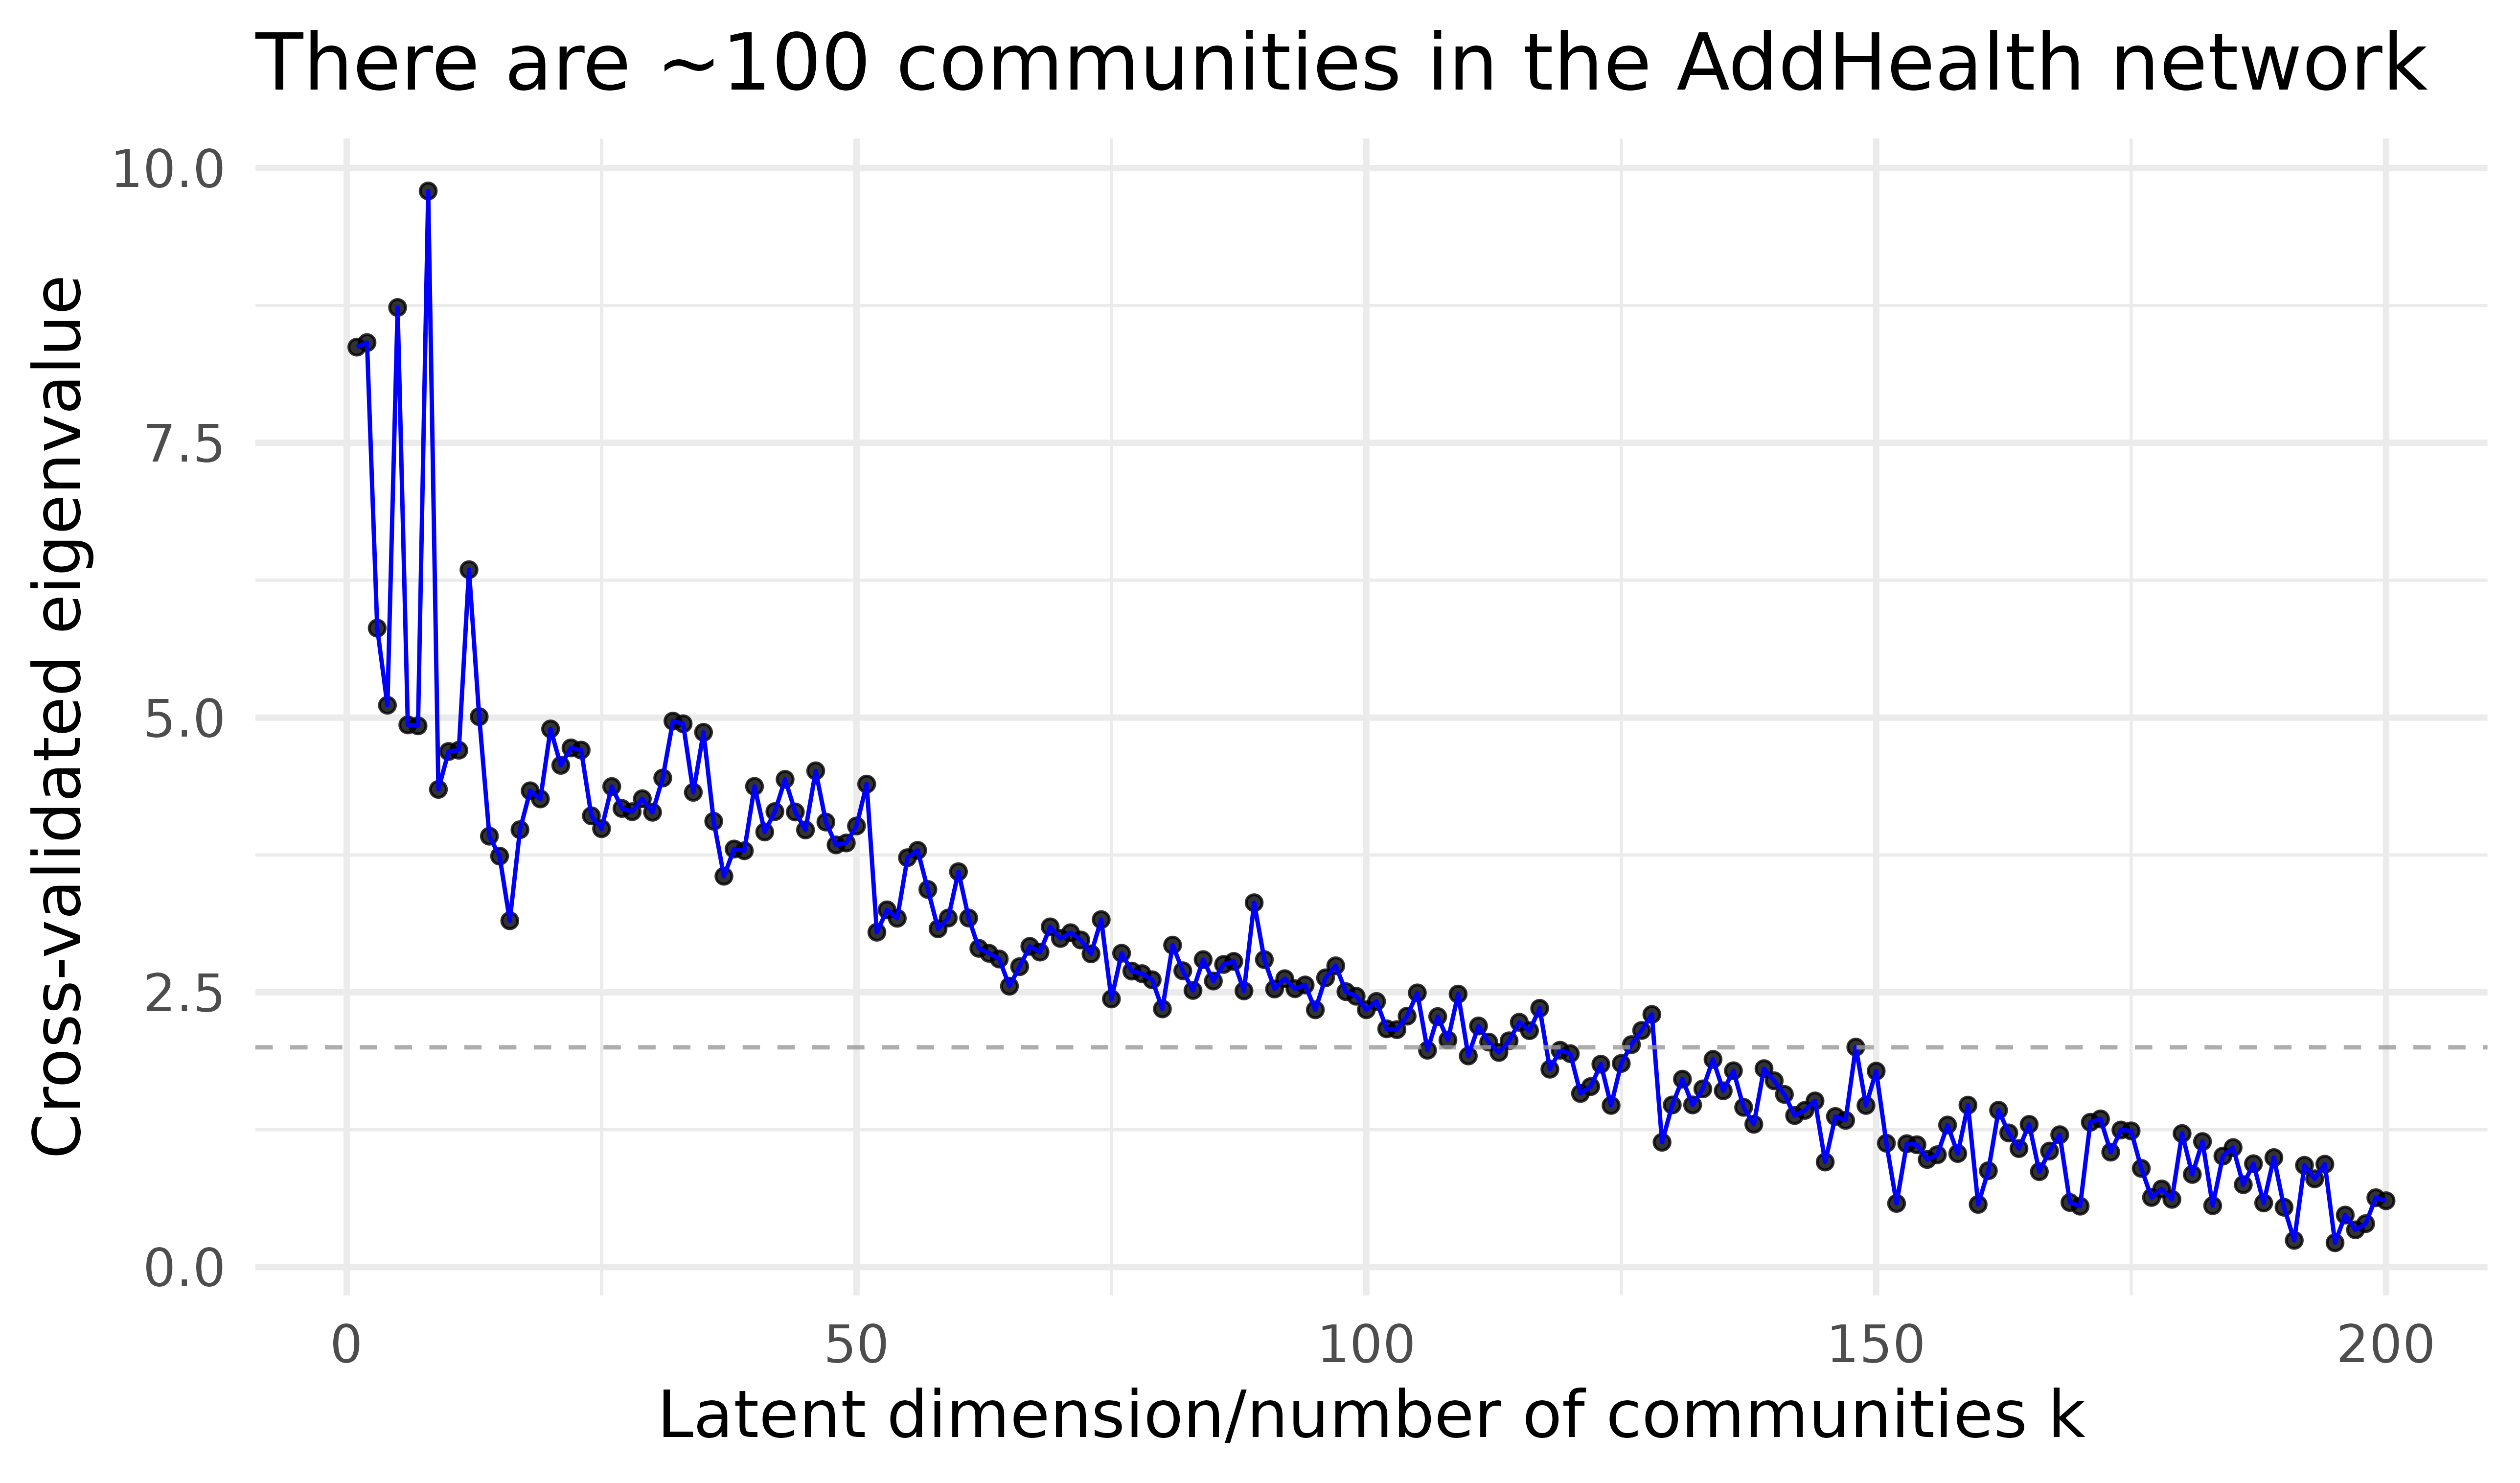
\includegraphics[width=0.9\textwidth]{figures/presentation/rank.png}
        \label{fig:rank}
    \end{figure}
\end{frame}

\begin{frame}{Mediated causal effects in the AddHealth data}

    \begin{figure}
        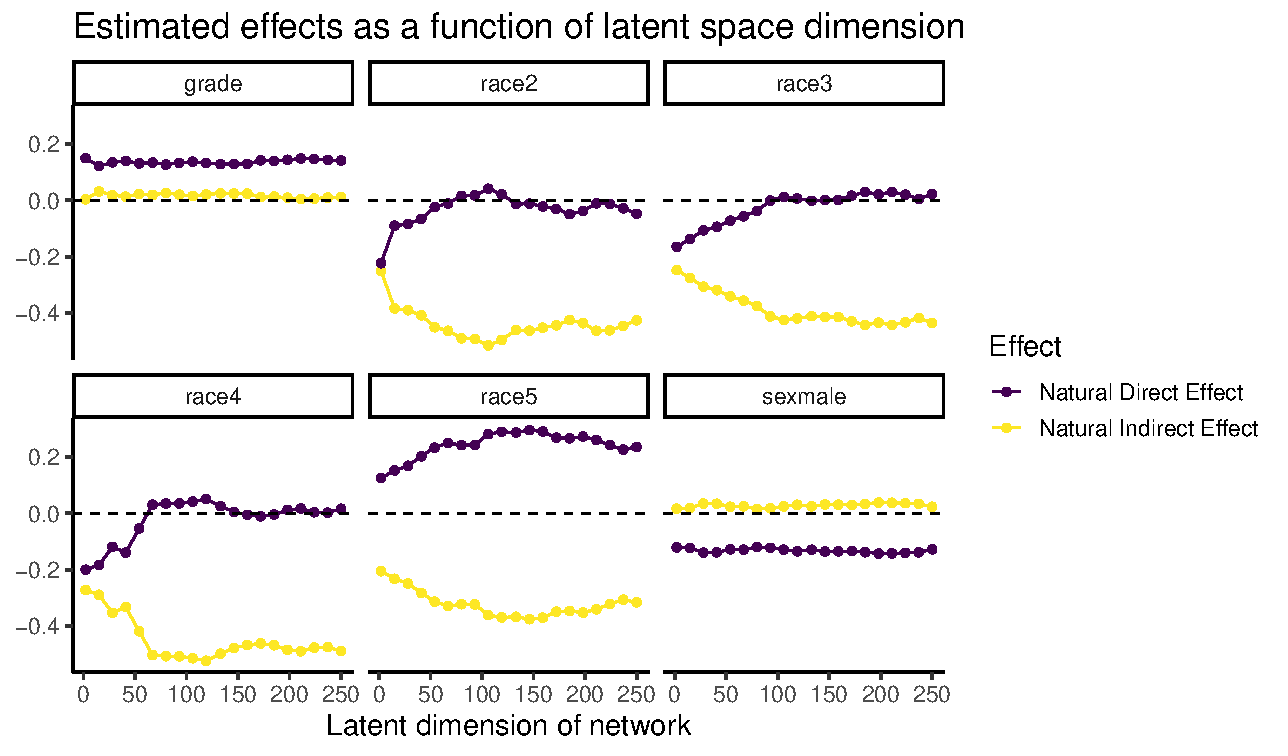
\includegraphics[width=\textwidth]{figures/addhealth-effects.pdf}
        \caption{Point estimates of natural direct and indirect effects in the AddHealth dataset as a function of varying embedding dimension $k$.}
        \label{fig:addhealth-estimates}
    \end{figure}
\end{frame}

\section{Thank you! Question?}

\begin{frame}{Interventions on a network}

    \begin{figure}
        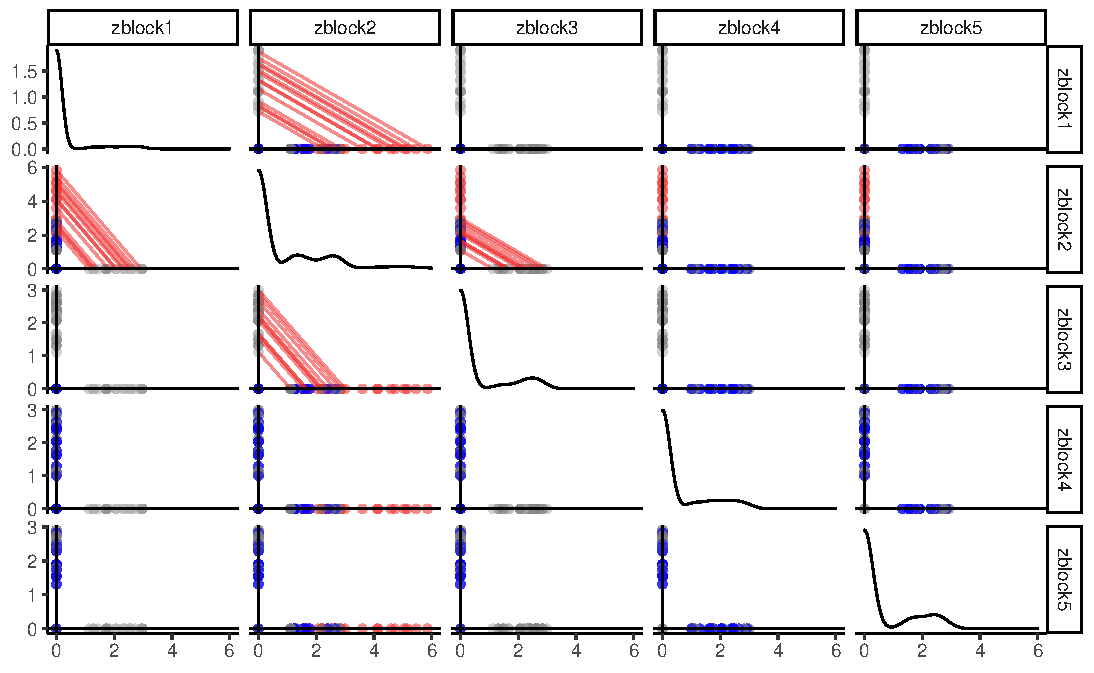
\includegraphics[width=\textwidth]{figures/intervention.pdf}
        \caption{Canonical intervention when $\C$ is highly informative.}
        \label{fig:intervention}
    \end{figure}
\end{frame}

\begin{frame}{Interventions on a network}

    \begin{align*}
        \underbrace{\E[T, \C]{\X}}_{\mathbb R^{1 \times k}}
         & = \underbrace{\thetazero}_{\mathbb R^{1 \times k}}
        + \underbrace{t}_{\{0, 1\}} \underbrace{\thetat}_{\mathbb R^{1 \times k}}
        + \underbrace{\c}_{\mathbb R^{1 \times p}} \underbrace{\Thetac}_{\mathbb R^{p \times k}},
        + \underbrace{t}_{\{0, 1\}} \underbrace{\c}_{\mathbb R^{1 \times p}} \underbrace{\Thetatc}_{\mathbb R^{p \times k}}
    \end{align*}

    In Figure \ref{fig:intervention}, $\C$ are latent parameters for a DC-SBM and $\thetazero = \vec 0, \thetat = \vec 0, \Thetac = I_k$ and

    \begin{align*}
        \Thetatc =
        \begin{bmatrix}
            -1 & 2 & 0  & 0 & 0 \\
            0  & 0 & 0  & 0 & 0 \\
            0  & 1 & -1 & 0 & 0 \\
            0  & 0 & 0  & 0 & 0 \\
            0  & 0 & 0  & 0 & 0 \\
        \end{bmatrix}
    \end{align*}
\end{frame}

\begin{frame}{Overcontrol bias from causal misspecification}

    When $\X$ is a mediator

    \begin{align*}
        \paren*{t - t^*} \, \betat = \nde = \ate - \nie
    \end{align*}

    When $\X$ is a confounder

    \begin{align*}
        \paren*{t - t^*} \, \betat = \ate
    \end{align*}

\end{frame}

\begin{frame}{Abstract}

    The last several years have seen a renewed and concerted effort to incorporate network data into standard tools for regression analysis, and to make network-linked data legible to practicing scientists. Thus far, this literature has primarily developed tools to infer associative relationships between nodal covariates and network structure. In contrast, we augment a statistical model for network regression with counterfactual assumptions and show how causal effects on a network can be partitioned into a direct effect that is uninfluenced by the network, and an indirect effect that is induced by homophily. The method is a conceptually straightforward integration of random dot product models for networks into the well-known product-of-coefficients mediation estimator.

\end{frame}

\bibliographystyle{chicago}
\bibliography{references}

\end{document}